%counter_example_tikz.tex

\begin{figure*}[t]
  \centering
  \begin{subfigure}[c]{0.5\textwidth}
 %   \centering
    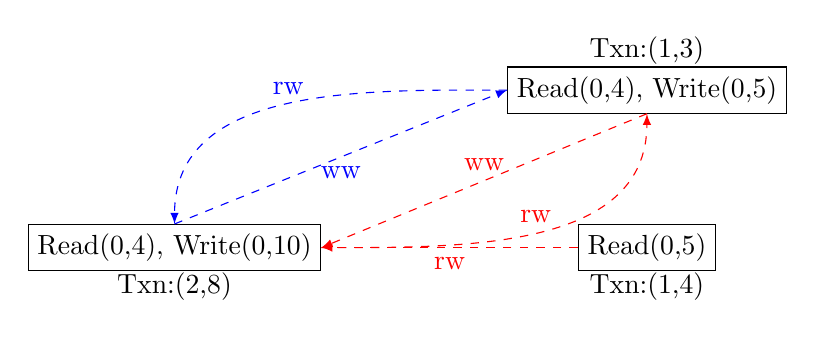
\begin{tikzpicture}[model/.style = {draw, minimum size = 15pt},  node distance = 0.5cm and 1.5cm]
        \node[model] (13) at (6,2) {Read(0,4), Write(0,5)};
        \node (textof13) at (6,2.5) {Txn:(1,3)};
        \node[model] (28) at (0,0) {Read(0,4), Write(0,10)};
        \node (textof28) at (0,-0.5) {Txn:(2,8)};
        \node[model] (14) at (6,0) {Read(0,5)};
        \node (textof14) at (6,-0.5) {Txn:(1,4)};
        \path[dashed, -latex, color=red] (13.south) edge node[above] {ww} (28.east); 
        \path[dashed, -latex, color=blue] (28.north) edge node[below] {ww} (13.west); 
        \path[dashed, -latex, color=blue] (13.west) edge [out=180,in=90] node[above] {rw} (28.north);
        \path[dashed, -latex, color=red] (28.east) edge [out=0,in=-90] node[above] {rw} (13.south);
        \path[dashed, -latex,color=red] (14.west) edge node[below] {rw} (28.east); 
    \end{tikzpicture}
    \caption{The original output of the violation in Galeta.}
    \label{fig:original-galera}
  \end{subfigure}
  
  \hfill
  
  \begin{subfigure}[c]{0.5\textwidth}
 %   \centering
    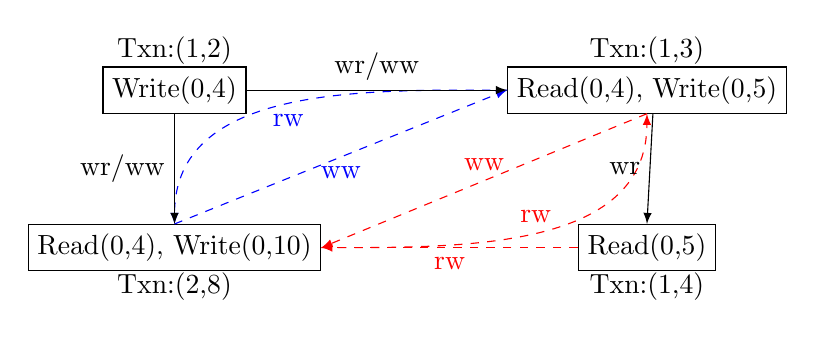
\begin{tikzpicture}[model/.style = {draw, minimum size = 15pt},  node distance = 0.5cm and 1.5cm]
        \node[model] (13) at (6,2) {Read(0,4), Write(0,5)};
        \node (textof13) at (6,2.5) {Txn:(1,3)};
        \node[model] (28) at (0,0) {Read(0,4), Write(0,10)};
        \node (textof28) at (0,-0.5) {Txn:(2,8)};
        \node[model] (14) at (6,0) {Read(0,5)};
        \node (textof14) at (6,-0.5) {Txn:(1,4)};
        \node[model] (12) at (0,2) {Write(0,4)};
        \node (textof12) at (0,2.5) {Txn:(1,2)};
        \path[dashed, -latex, color=red] (13.south) edge node[above] {ww} (28.east); 
        \path[dashed, -latex, color=blue] (28.north) edge node[below] {ww} (13.west); 
        \path[dashed, -latex, color=blue] (13.west) edge [out=180,in=90] node[below] {rw} (28.north);
        \path[dashed, -latex, color=red] (28.east) edge [out=0,in=-90] node[above] {rw} (13.south);
        \path[dashed, -latex,color=red] (14.west) edge node[below] {rw} (28.east); 
        \path[-latex] (12.east) edge node[above] {wr/ww} (13.west);
        \path[-latex] (12.south) edge node[left] {wr/ww} (28.north);
        \path[-latex] ([xshift=0.5ex]13.south) edge node[left] {wr} (14.north);
    \end{tikzpicture}
    \caption{Recover the information.}
    \label{fig:recover-galera}
  \end{subfigure}
  
  \hfill
  
  \begin{subfigure}[c]{0.5\textwidth}
 %   \centering
    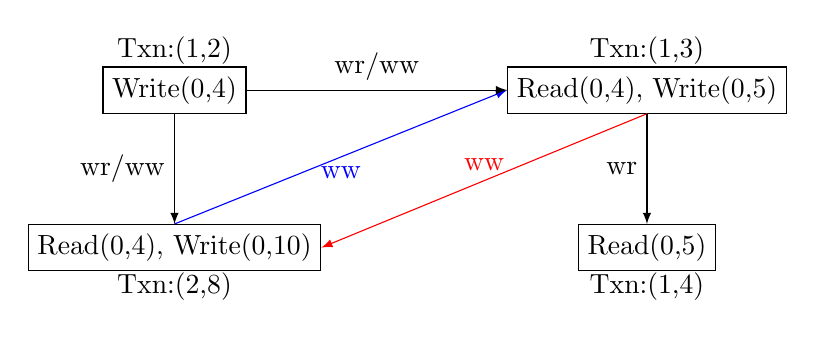
\begin{tikzpicture}[model/.style = {draw, minimum size = 15pt},  node distance = 0.5cm and 1.5cm]
        \node[model] (13) at (6,2) {Read(0,4), Write(0,5)};
        \node (textof13) at (6,2.5) {Txn:(1,3)};
        \node[model] (28) at (0,0) {Read(0,4), Write(0,10)};
        \node (textof28) at (0,-0.5) {Txn:(2,8)};
        \node[model] (14) at (6,0) {Read(0,5)};
        \node (textof14) at (6,-0.5) {Txn:(1,4)};
        \node[model] (12) at (0,2) {Write(0,4)};
        \node (textof12) at (0,2.5) {Txn:(1,2)};
        \path[-latex, color=red] (13.south) edge node[above] {ww} (28.east); 
        \path[-latex, color=blue] (28.north) edge node[below] {ww} (13.west); 
        \path[-latex] (12.east) edge node[above] {wr/ww} (13.west);
        \path[-latex] (12.south) edge node[left] {wr/ww} (28.north);
        \path[-latex] (13.south) edge node[left] {wr} (14.north);
    \end{tikzpicture}
    \caption{Delete uncertainty.}
    \label{fig:delete-galera}
  \end{subfigure}
  \label{fig:counter_example_galera}
  \caption{Counter example of Galera}
\end{figure*}

\begin{figure*}[t]
  \centering
  \begin{subfigure}[c]{0.5\textwidth}
 %   \centering
    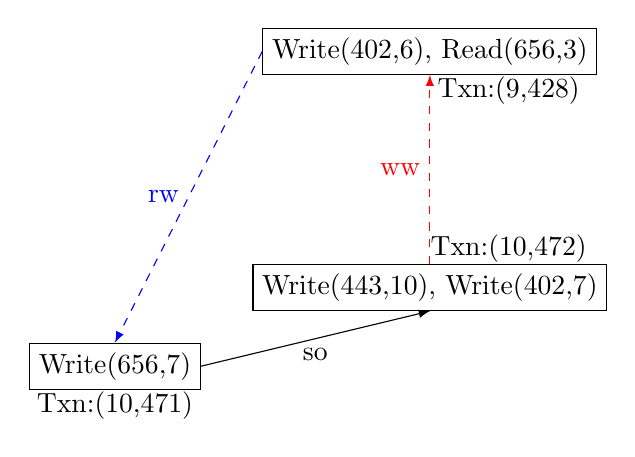
\begin{tikzpicture}[model/.style = {draw, minimum size = 15pt},  node distance = 0.5cm and 1.5cm]
        \node[model] (10472) at (0,0) {Write(443,10), Write(402,7)};
        \node (textof10472) at (1,0.5) {Txn:(10,472)};
        \node[model] (9428) at (0,3) {Write(402,6), Read(656,3)};
        \node (textof9428) at (1,2.5) {Txn:(9,428)};
        \node[model] (10471) at (-4,-1) {Write(656,7)};
        \node (textof10471) at (-4,-1.5) {Txn:(10,471)};
        \path[dashed, -latex, color=red] (10472.north) edge node[left] {ww} (9428.south); 
        \path[dashed, -latex, color=blue] (9428.west) edge node[left] {rw} (10471.north); 
        \path[-latex] (10471.east) edge node[below] {so} (10472.south); 
    \end{tikzpicture}
    \caption{The original output of the violation in DGraph.}
    \label{fig:original-DGraph}
  \end{subfigure}
  
  \hfill
  
  \begin{subfigure}[c]{0.5\textwidth}
 %   \centering
  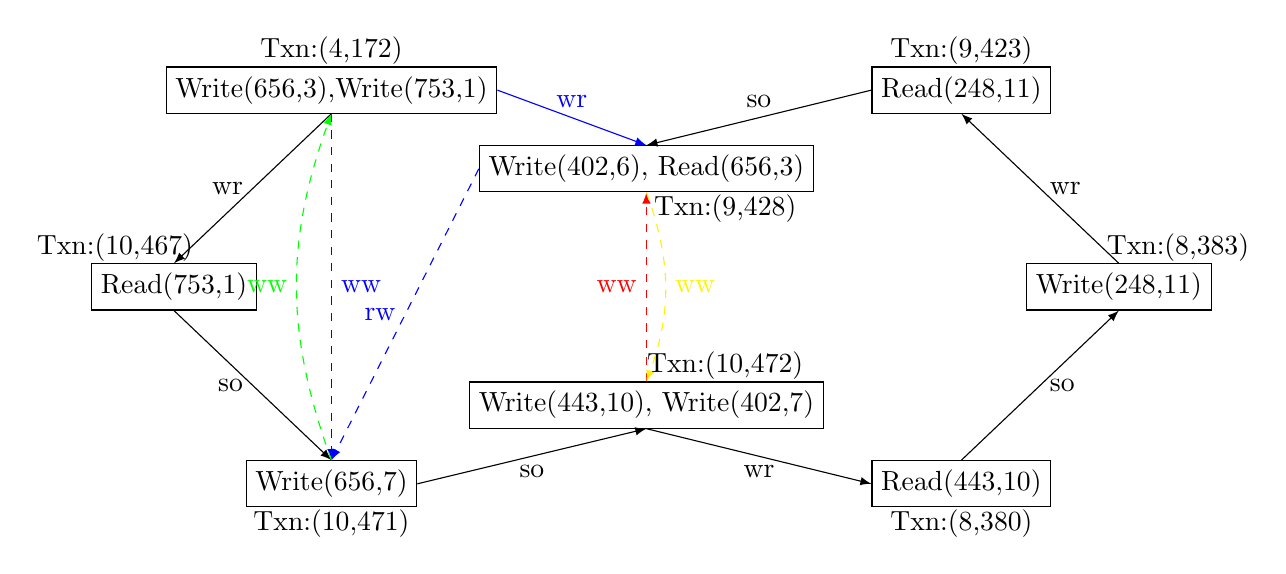
\begin{tikzpicture}[model/.style = {draw, minimum size = 15pt},  node distance = 0.5cm and 1.5cm]
        \node[model] (10472) at (0,0) {Write(443,10), Write(402,7)};
        \node (textof10472) at (1,0.5) {Txn:(10,472)};
        \node[model] (9428) at (0,3) {Write(402,6), Read(656,3)};
        \node (textof9428) at (1,2.5) {Txn:(9,428)};
        \node[model] (10471) at (-4,-1) {Write(656,7)};
        \node (textof10471) at (-4,-1.5) {Txn:(10,471)};
        \node[model] (4172) at (-4,4) {Write(656,3),Write(753,1)};
        \node (textof4172) at (-4,4.5) {Txn:(4,172)};
        \node[model] (10467) at (-6,1.5) {Read(753,1)};
        \node (textof10467) at (-6.75,2) {Txn:(10,467)};
        \node[model] (8380) at (4,-1) {Read(443,10)};
        \node (textof8380) at (4,-1.5) {Txn:(8,380)};
        \node[model] (8383) at (6,1.5) {Write(248,11)};
        \node (textof8383) at (6.75,2) {Txn:(8,383)};
        \node[model] (9423) at (4,4) {Read(248,11)};
        \node (textof9423) at (4,4.5) {Txn:(9,423)};

        
        \path[dashed, -latex, color=red] (10472.north) edge node[left] {ww} (9428.south); 
        \path[dashed, -latex, color=blue] (9428.west) edge node[left] {rw} (10471.north); 
        \path[-latex] (10471.east) edge node[below] {so} (10472.south); 
        \path[-latex, color=blue] (4172.east) edge node[above] {wr} (9428.north) ; 
        \path[-latex] (4172.south) edge node[left] {wr} (10467.north); 
        \path[-latex] (10467.south) edge node[left] {so} (10471.north); 
        \path[-latex] (10472.south) edge node[below] {wr} (8380.west); 
        \path[-latex] (8380.north) edge node[right] {so} (8383.south); 
        \path[-latex] (8383.north) edge node[right] {wr} (9423.south);
        \path[-latex] (9423.west) edge node[above] {so} (9428.north);
        
        \path[dashed, -latex, color=blue] (4172.south) edge node[right] {ww} (10471.north) ; 
        \path[dashed, -latex, color=green] (10471.north)  edge [out=110,in=-110] node[left] {ww}  (4172.south) ; 
        \path[dashed, -latex, color=yellow] (9428.south)  edge [out=-70,in=70] node[right] {ww}  (10472.north) ;
    \end{tikzpicture}
    \caption{Recover the information.}
    \label{fig:recover-DGraph}
  \end{subfigure}
  
  \hfill
  
  \begin{subfigure}[c]{0.5\textwidth}
 %   \centering
  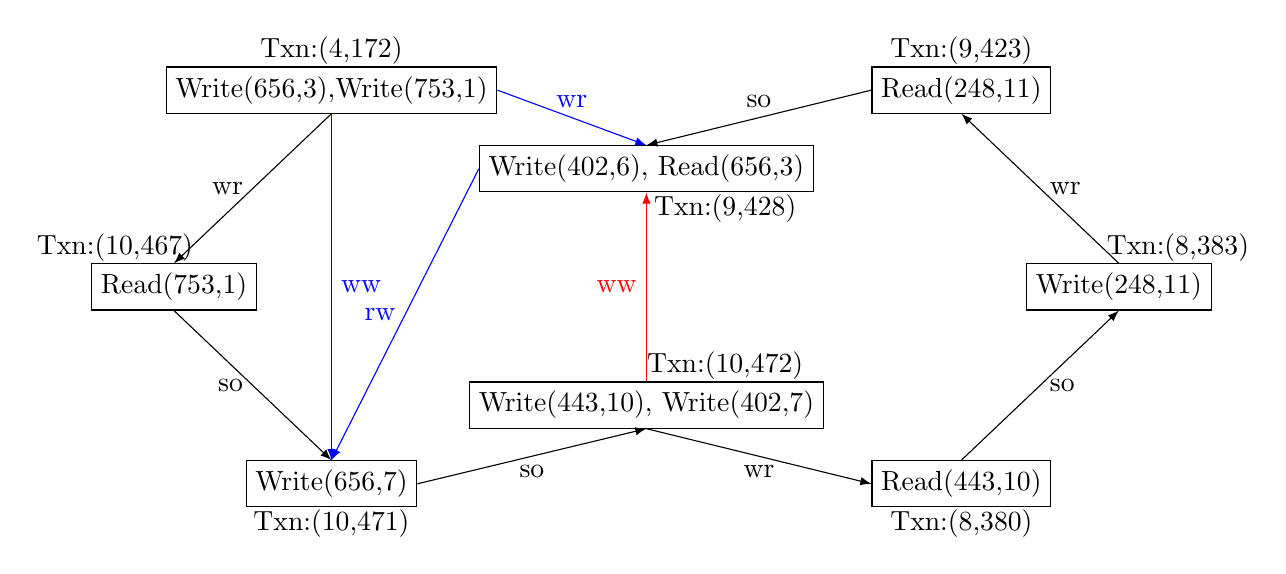
\begin{tikzpicture}[model/.style = {draw, minimum size = 15pt},  node distance = 0.5cm and 1.5cm]
        \node[model] (10472) at (0,0) {Write(443,10), Write(402,7)};
        \node (textof10472) at (1,0.5) {Txn:(10,472)};
        \node[model] (9428) at (0,3) {Write(402,6), Read(656,3)};
        \node (textof9428) at (1,2.5) {Txn:(9,428)};
        \node[model] (10471) at (-4,-1) {Write(656,7)};
        \node (textof10471) at (-4,-1.5) {Txn:(10,471)};
        \node[model] (4172) at (-4,4) {Write(656,3),Write(753,1)};
        \node (textof4172) at (-4,4.5) {Txn:(4,172)};
        \node[model] (10467) at (-6,1.5) {Read(753,1)};
        \node (textof10467) at (-6.75,2) {Txn:(10,467)};
        \node[model] (8380) at (4,-1) {Read(443,10)};
        \node (textof8380) at (4,-1.5) {Txn:(8,380)};
        \node[model] (8383) at (6,1.5) {Write(248,11)};
        \node (textof8383) at (6.75,2) {Txn:(8,383)};
        \node[model] (9423) at (4,4) {Read(248,11)};
        \node (textof9423) at (4,4.5) {Txn:(9,423)};

        
        \path[-latex, color=red] (10472.north) edge node[left] {ww} (9428.south); 
        \path[-latex, color=blue] (9428.west) edge node[left] {rw} (10471.north); 
        \path[-latex] (10471.east) edge node[below] {so} (10472.south); 
        \path[-latex, color=blue] (4172.east) edge node[above] {wr} (9428.north) ; 
        \path[-latex] (4172.south) edge node[left] {wr} (10467.north); 
        \path[-latex] (10467.south) edge node[left] {so} (10471.north); 
        \path[-latex] (10472.south) edge node[below] {wr} (8380.west); 
        \path[-latex] (8380.north) edge node[right] {so} (8383.south); 
        \path[-latex] (8383.north) edge node[right] {wr} (9423.south);
        \path[-latex] (9423.west) edge node[above] {so} (9428.north);
        
        \path[-latex, color=blue] (4172.south) edge node[right] {ww} (10471.north) ;  (10472.north) ;
    \end{tikzpicture}
    \caption{Delete uncertainty.}
    \label{fig:delete-DGraph}
  \end{subfigure}
  \caption{Counter example of DGraph}
  \label{fig:counter_example_DGraph}
\end{figure*}


\begin{figure*}[t]
  \centering
  \begin{subfigure}[c]{0.5\textwidth}
 %   \centering
    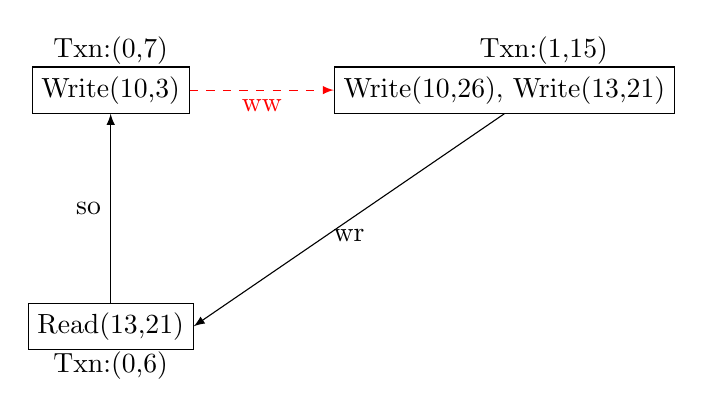
\begin{tikzpicture}[model/.style = {draw, minimum size = 15pt},  node distance = 0.5cm and 1.5cm]
        \node[model] (07) at (0,0) {Write(10,3)};
        \node (textof07) at (0,0.5) {Txn:(0,7)};
        \node[model] (06) at (0,-3) {Read(13,21)};
        \node (textof06) at (0,-3.5) {Txn:(0,6)};
        \node[model] (115) at (5,0) {Write(10,26), Write(13,21)};
        \node (textof115) at (5.5,0.5) {Txn:(1,15)};
        
        \path[dashed, -latex, color=red] (07.east) edge node[below] {ww} (115.west); 
        \path[-latex] (06.north) edge node[left] {so} (07.south); 
        \path[-latex] (115.south) edge node[below] {wr} (06.east); 
    \end{tikzpicture}
    \caption{The original output of the violation in DGraph.}
    \label{fig:original-yuga}
  \end{subfigure}
  
  \hfill
  
  \begin{subfigure}[c]{0.5\textwidth}
 %   \centering
    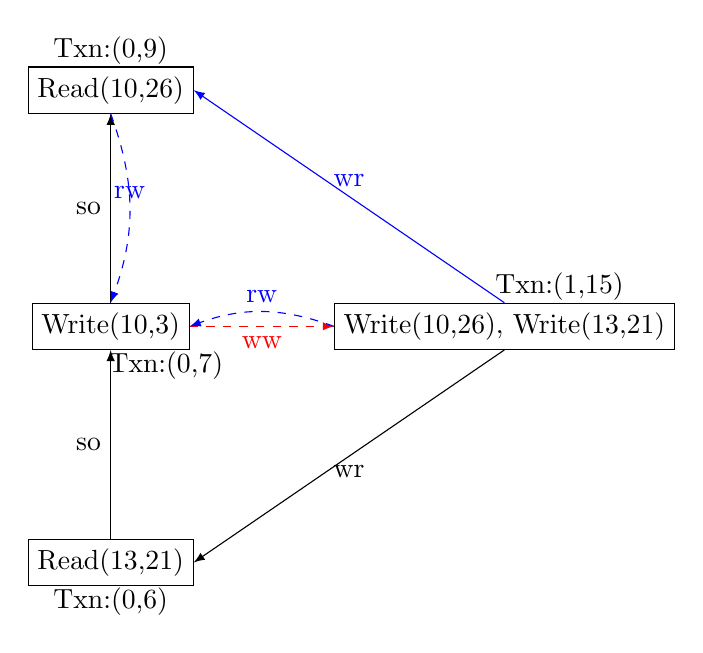
\begin{tikzpicture}[model/.style = {draw, minimum size = 15pt},  node distance = 0.5cm and 1.5cm]
        \node[model] (07) at (0,0) {Write(10,3)};
        \node (textof07) at (0.7,-0.5) {Txn:(0,7)};
        \node[model] (06) at (0,-3) {Read(13,21)};
        \node (textof06) at (0,-3.5) {Txn:(0,6)};
        \node[model] (115) at (5,0) {Write(10,26), Write(13,21)};
        \node (textof115) at (5.7,0.5) {Txn:(1,15)};
        \node[model] (09) at (0,3) {Read(10,26)};
        \node (textof09) at (0,3.5) {Txn:(0,9)};
        
        \path[dashed, -latex, color=red] (07.east) edge node[below] {ww} (115.west); 
        \path[-latex] (06.north) edge node[left] {so} (07.south); 
        \path[-latex] (115.south) edge node[below] {wr} (06.east); 
        \path[-latex] (07.north) edge node[left] {so} (09.south); 
        \path[-latex,color=blue] (115.north) edge node[above] {wr} (09.east); 
        \path[dashed, -latex,color=blue] (09.south) edge [out=-70,in=70] node[above] {rw} (07.north); 
        \path[dashed, -latex,color=blue] (115.west) edge [out=160,in=20] node[above] {rw} (07.east); 
    \end{tikzpicture}
    \caption{Recover the information.}
    \label{fig:recover-yuga}
  \end{subfigure}
  
  \hfill
  
  \begin{subfigure}[c]{0.5\textwidth}
 %   \centering
    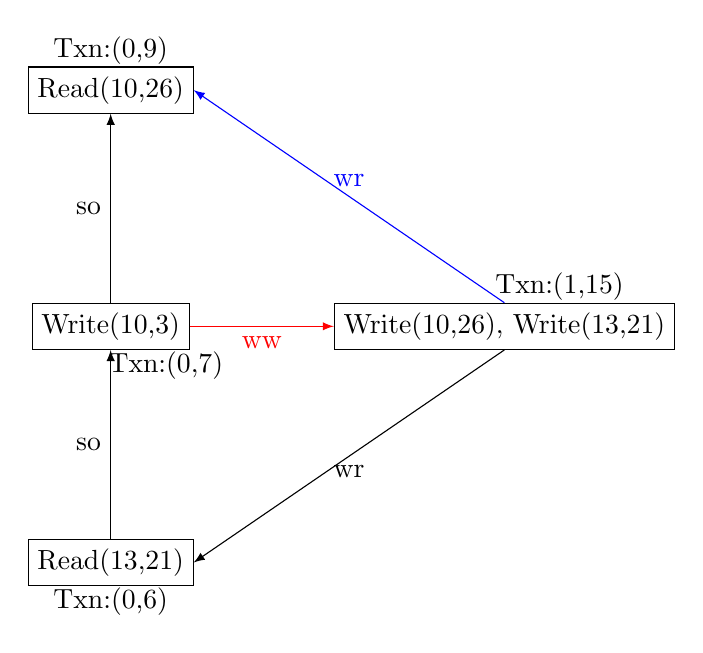
\begin{tikzpicture}[model/.style = {draw, minimum size = 15pt},  node distance = 0.5cm and 1.5cm]
        \node[model] (07) at (0,0) {Write(10,3)};
        \node (textof07) at (0.7,-0.5) {Txn:(0,7)};
        \node[model] (06) at (0,-3) {Read(13,21)};
        \node (textof06) at (0,-3.5) {Txn:(0,6)};
        \node[model] (115) at (5,0) {Write(10,26), Write(13,21)};
        \node (textof115) at (5.7,0.5) {Txn:(1,15)};
        \node[model] (09) at (0,3) {Read(10,26)};
        \node (textof09) at (0,3.5) {Txn:(0,9)};
        
        \path[-latex, color=red] (07.east) edge node[below] {ww} (115.west); 
        \path[-latex] (06.north) edge node[left] {so} (07.south); 
        \path[-latex] (115.south) edge node[below] {wr} (06.east); 
        \path[-latex] (07.north) edge node[left] {so} (09.south); 
        \path[-latex,color=blue] (115.north) edge node[above] {wr} (09.east); 
    \end{tikzpicture}
    \caption{Delete uncertainty.}
    \label{fig:delete-yuga}
  \end{subfigure}
  
  \caption{Counter example of Yuga}
  \label{fig:counter_example_DGraph}
\end{figure*}
